\documentclass[10pt]{beamer}

\usetheme{Madrid}
\usecolortheme{default}

% Base packages
%\usepackage{helvet}
\usepackage{amsmath,amssymb,mathtools,subcaption}
\usepackage{tikz,pgfplots,tabularx,booktabs}
\usepackage{listings}
\usepackage{xcolor}

% Font settings
\renewcommand{\familydefault}{\sfdefault}

% TikZ libraries
\usetikzlibrary{calc,positioning,backgrounds,decorations.pathreplacing}
\pgfplotsset{compat=1.14}

% Colors
\definecolor{deepblue}{RGB}{42,39,155}
\definecolor{lightpink}{RGB}{255,240,240}
\definecolor{lightgreen}{RGB}{240,255,240}
\definecolor{lightyellow}{RGB}{255,255,240}
\definecolor{codegray}{RGB}{245,245,245}
\definecolor{codegreen}{rgb}{0,0.6,0}
\definecolor{codepurple}{rgb}{0.58,0,0.82}

% Beamer settings
\setbeamercolor{title}{fg=white,bg=deepblue}
\setbeamercolor{frametitle}{fg=white,bg=deepblue}
\setbeamercolor{section in head/foot}{fg=white,bg=deepblue}

% Code listing settings
\lstdefinelanguage{iPython}{
  language=Python,
  morekeywords={as,assert,async,await,break,class,continue,def,del,elif,else,
    except,finally,for,from,global,if,import,in,is,lambda,nonlocal,not,or,
    pass,raise,return,try,while,with,yield,True,False,None},
  sensitive=true,
  morecomment=[l]{\#},
  morestring=[b]',
  morestring=[b]"
}

\lstset{
    language=iPython,
    basicstyle=\ttfamily\small,
    backgroundcolor=\color{codegray},
    breaklines=true,
    showstringspaces=false,
    commentstyle=\color{codegreen},
    keywordstyle=\color{blue},
    stringstyle=\color{codepurple},
    numbers=none,
    frame=none
}

\setbeamertemplate{footline}[text line]{%
  \parbox{\linewidth}{\vspace*{-8pt}
  %\hfill\href{https://github.com/chang-ye-tu/fin}{https://github.com/chang-ye-tu/fin}
    \hfill
   ~~ \insertframenumber / \inserttotalframenumber~~~~~~~~~}}
\setbeamertemplate{navigation symbols}{}%[only frame symbol]

\definecolor{foo}{rgb}{.2,.2,.7}
\AtBeginSection[]{
  \begin{frame}
  \vfill
  \centering
  \begin{beamercolorbox}[sep=8pt,center,shadow=true,rounded=true]{section page}
    \usebeamerfont{title}%
    {\color{foo} \insertsectionhead}\par%
  \end{beamercolorbox}
  \vfill
  \end{frame}
}

\title{Introduction to Financial Models \\ Lecture 01: Surprises \& Paradoxes I}
\author{}
\date{}

\begin{document}

\begin{frame}
\titlepage
\end{frame}

\subsection*{Outline}
\begin{frame}
  \tableofcontents
\end{frame}

\section{Simpson Paradox}

\begin{frame}
\begin{table}[!htbp]
  \centering
  \begin{tabular}{lcccccc}
    \toprule
    & \multicolumn{3}{c}{Women} & \multicolumn{3}{c}{Men} \\
    & applied & accepted & \% & applied & accepted & \% \\
    \midrule
    Computer Science & 26 & 7 & 27 & 228 & 58 & 25 \\
    Economics & 240 & 63 & 26 & 512 & 112 & 22 \\
    Engineering & 164 & 52 & 32 & 972 & 252 & 26 \\
    Medicine & 416 & 99 & 24 & 578 & 140 & 24 \\
    Veterinary medicine & 338 & 53 & 16 & 180 & 22 & 12 \\
    \midrule
    Total & 1184 & 274 & 23 & 2470 & 584 & 24 \\
    \bottomrule
  \end{tabular}
  \caption{Cambridge University Admission Data, 1996.}
  \label{fig:simpson}
\end{table}
\end{frame}

\section{Data Morph: A Guided Tour}

\begin{frame}{Milestones}
\begin{itemize}%\setlength\itemsep{0em}
  \item\href{https://en.wikipedia.org/wiki/Anscombe\%27s_quartet}{Anscombe, F., 1973. Anscombe's Quartet.}
  \item\href{https://en.wikipedia.org/wiki/Datasaurus_dozen}{Cairo, A., 2016. Datasaurus Dozen} 
  \item Matejka, J., Fitzmaurice, G., 2017. Same Stats, Different Graphs: Generating Datasets with Varied Appearance and Identical Statistics through Simulated Annealing. \href{https://www.research.autodesk.com/publications/same-stats-different-graphs/}{Website}, \href{https://research.autodesk.com/app/uploads/2023/03/same-stats-different-graphs.pdf_rec2hRjLLGgM7Cn2T.pdf}{Paper}, \href{https://github.com/jmatejka/same-stats-different-graphs}{Code}, \href{https://www.youtube.com/watch?v=DbJyPELmhJc}{YouTube}
  \item Molin, S., 2024. Data Morph: Moving Beyond the Datasaurus Dozen. \href{https://stefaniemolin.com/articles/data-science/introducing-data-morph/}{Website}, \href{https://github.com/stefmolin/data-morph}{Code}.
\end{itemize}
\end{frame}

\begin{frame}
  Let's play a game. I'm thinking of a distribution with the following summary statistics. Can you picture what a scatter plot of the data would look like?
  \vspace{5mm}
  \begin{itemize}
    \item $X$ mean = 30.37
    \item $Y$ mean = 53.01
    \item $X$ standard deviation = 13.44
    \item $Y$ standard deviation = 15.53
    \item Correlation coefficient = 0.04
  \end{itemize}
\end{frame}

\begin{frame}
  \begin{figure}
  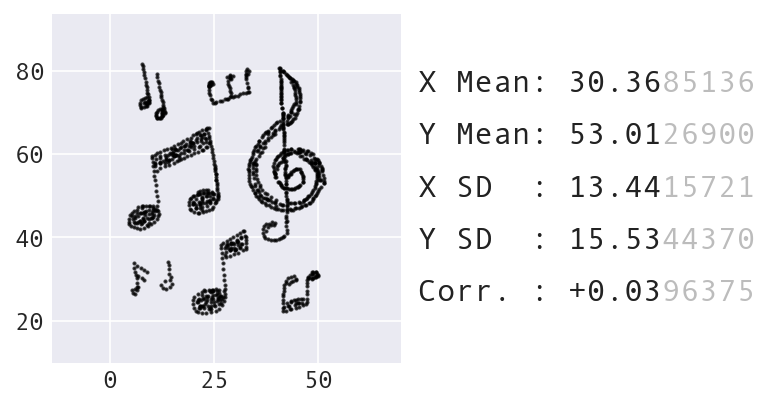
\includegraphics[width=.95\textwidth]{fig/note01/music-dataset.png}
  %\caption{Generated using different values of $\alpha$}
  \end{figure}
\end{frame}

\begin{frame}
  \begin{figure}
    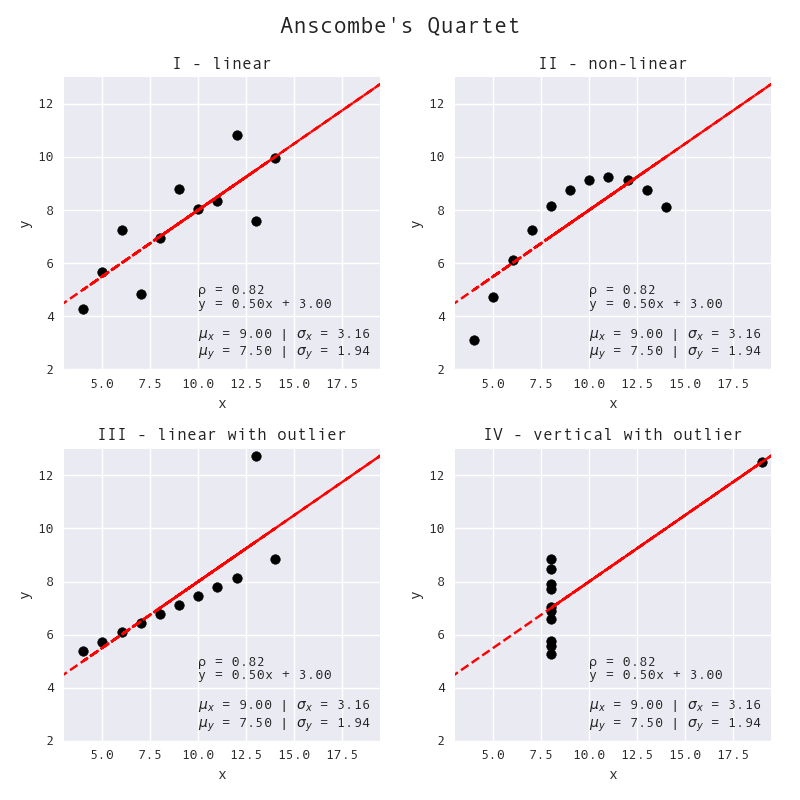
\includegraphics[height=.95\textheight]{fig/note01/anscombes-quartet.png}
  %\caption{Generated using different values of $\alpha$}
  \end{figure}
\end{frame}

\begin{frame}
  \begin{figure}
    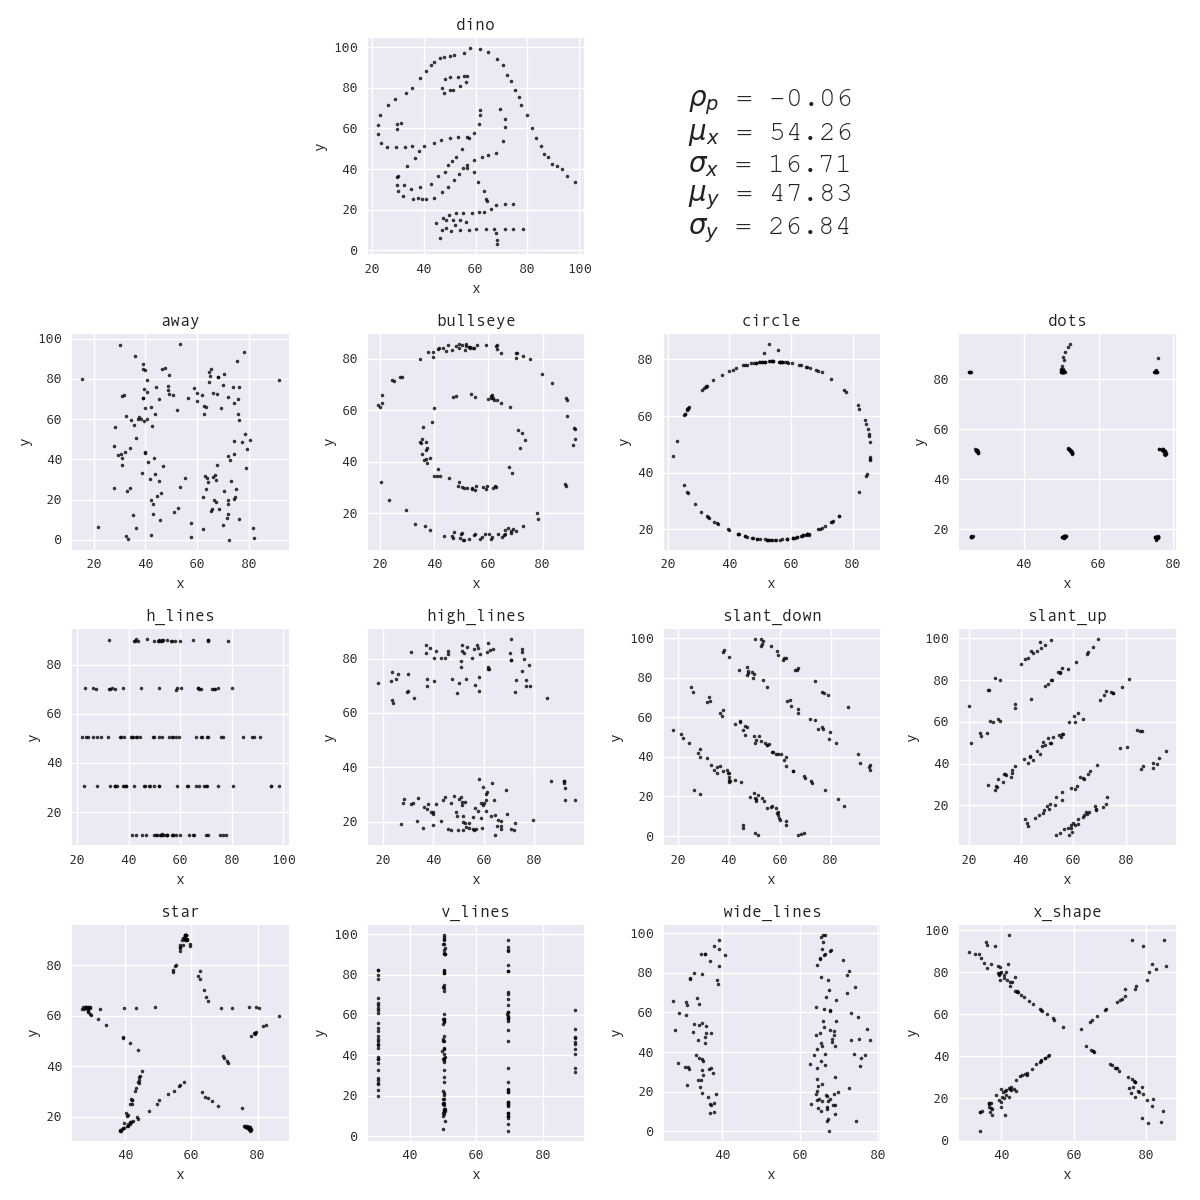
\includegraphics[height=.95\textheight]{fig/note01/datasaurus-dozen.png}
  %\caption{Generated using different values of $\alpha$}
  \end{figure}
\end{frame}

\begin{frame}{Data Morph}
  \begin{center}
    Demonstration: \href{https://www.research.autodesk.com/app/uploads/2023/03/DinoSequential-1.gif}{Datasaurus Dozen}, \href{https://stefaniemolin.com/assets/articles/data-science/introducing-data-morph/panda-to-star.gif}{Panda to Star}, \href{https://twitter.com/StefanieMolin/status/1645046652971933696}{Happy Easter}
  \end{center}
\end{frame}

\section{How to Fit Any Dataset with a Single Parameter}

\begin{frame}{The Core Result}

Boué, L., 2019. Real Numbers, Data Science and Chaos: How to Fit any Dataset with a Single Parameter. \href{https://arxiv.org/abs/1904.12320}{arXiv}, \href{https://github.com/Ranlot/single-parameter-fit}{Code.}
\vspace{5mm}

Main theorem: Any dataset can be fit using
\[ f_\alpha(x) = \sin^2(2^{x\tau} \arcsin\sqrt{\alpha}) \]
where:
\begin{itemize}
\item $\alpha \in \mathbb{R}$ is a single learned parameter
\item $x \in [0,\cdots,n]$ takes integer values
\item $\tau \in \mathbb{N}$ controls accuracy
\end{itemize}

Properties:
\begin{itemize}
\item Continuous and differentiable
\item Arbitrary precision fit
\item Single real-valued parameter
\end{itemize}
\end{frame}

\begin{frame}{Demonstration: Animal Shapes}
\begin{figure}
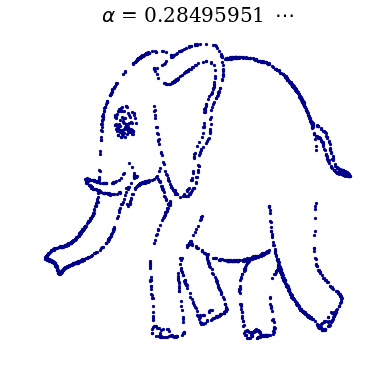
\includegraphics[width=0.24\textwidth]{fig/note01/elephant.png}
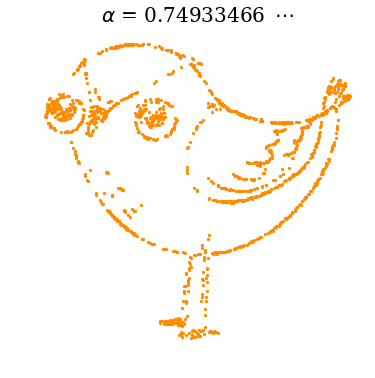
\includegraphics[width=0.24\textwidth]{fig/note01/bird.png}
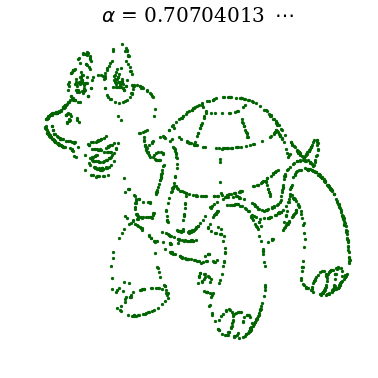
\includegraphics[width=0.24\textwidth]{fig/note01/turtle.png}
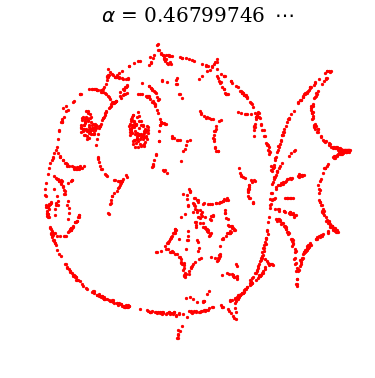
\includegraphics[width=0.24\textwidth]{fig/note01/fish.png}
\caption{Generated using different values of $\alpha$}
\end{figure}

\begin{itemize}
\item Each shape is a scatter plot $(x,y)$
\item $x \in \mathbb{N}$ are integer values
\item $y = f_\alpha(x)$ gives y-coordinates
\item Different $\alpha$ values = different shapes
\end{itemize}
\end{frame}

\begin{frame}{Audio Signal Example}
\begin{figure}
\begin{subfigure}{0.48\textwidth}
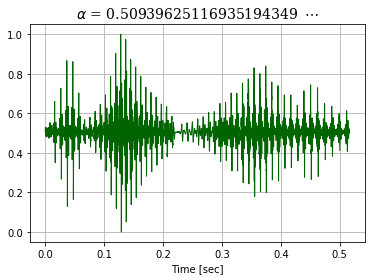
\includegraphics[width=\textwidth]{fig/note01/generated_waveform.png}
\caption{Waveform}
\end{subfigure}
\begin{subfigure}{0.48\textwidth}
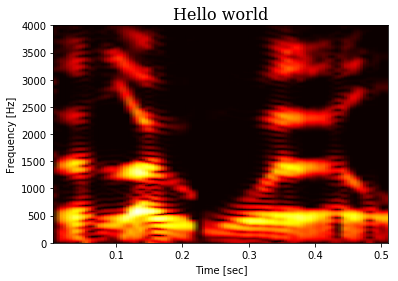
\includegraphics[width=\textwidth]{fig/note01/generated_spectrogram.png}
\caption{Spectrogram}
\end{subfigure}
\caption{"Hello world" audio signal}
\end{figure}

Processing:
\begin{itemize}
\item Sample at 11kHz
\item Values determined by $f_\alpha$
\item Complex waveform from single $\alpha$
\end{itemize}
\end{frame}

\begin{frame}{Fixed-point Binary Representation}
For $\alpha \in [0,1]$:
\[ \alpha = \sum_{n=1}^{+\infty} \frac{a_n}{2^n} \]
where $a_n \in \{0,1\}$

\begin{center}
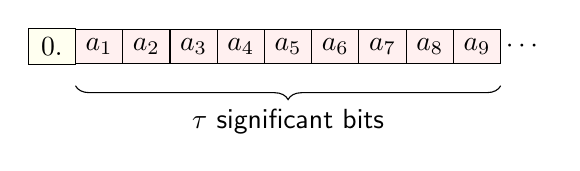
\begin{tikzpicture}[scale=1]
\node[draw,minimum width=0.6cm,fill=lightyellow] at (0,0) {$0.$};
\foreach \x in {1,...,9} {
    \node[draw,minimum width=0.6cm,fill=lightpink] at (0.6*\x,0) {$a_{\x}$};
}
\node at (6,0) {$\cdots$};

\draw[decorate,decoration={brace,mirror,amplitude=5pt}]
    (0.3,-.5) -- (5.7,-.5) 
    node[below,midway,yshift=-5pt] {$\tau$ significant bits};
\end{tikzpicture}
\end{center}

In practice:
\begin{itemize}
\item Truncate to $\tau$ bits
\item Error bound: $|\alpha - \alpha_{\text{approx}}| \leq \frac{1}{2^\tau}$
\end{itemize}
\end{frame}

\begin{frame}{The Dyadic Transformation}
Definition:
\[ \mathcal{D}(\alpha_k) = 2\alpha_k \bmod 1 \]

Properties:
\begin{itemize}
\item Maps [0,1] to itself
\item Piecewise linear
\item Exhibits chaos
\end{itemize}

\begin{figure}
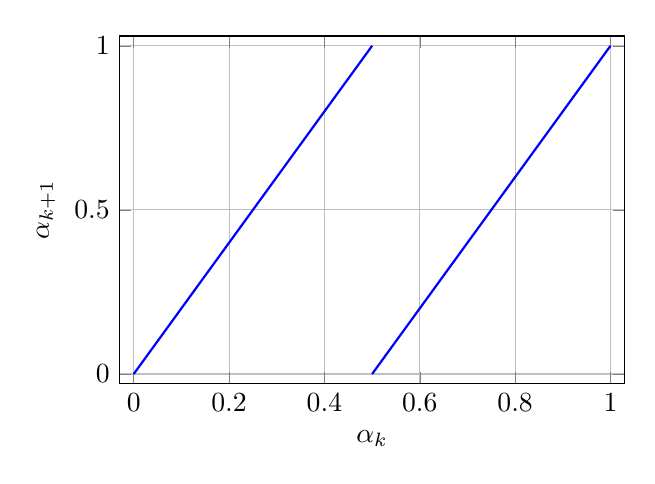
\begin{tikzpicture}
\begin{axis}[
    width=8cm, height=6cm,
    xmin=-0.03, xmax=1.03,
    ymin=-0.03, ymax=1.03,
    xlabel=$\alpha_k$,
    ylabel=$\alpha_{k+1}$,
    grid=both
]
\addplot[domain=0:0.5,samples=100,thick,blue]{2*x};
\addplot[domain=0.5:1,samples=100,thick,blue]{2*x-1};
\end{axis}
\end{tikzpicture}
\caption{Graph of $\mathcal{D}$}
\end{figure}
\end{frame}

\begin{frame}{Bit-Shift Property}
In binary, $\mathcal{D}$ is a left shift:

\begin{center}
  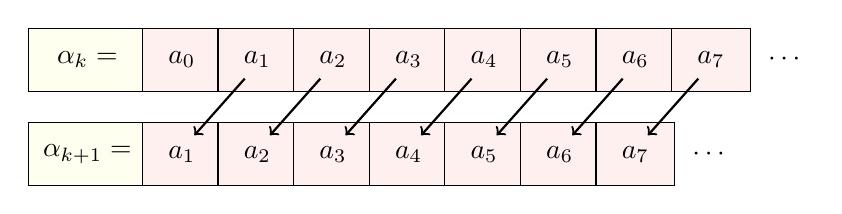
\begin{tikzpicture}[scale=0.8,
    box/.style={draw,minimum width=1cm,minimum height=0.8cm,fill=lightpink},
    labelbox/.style={draw,minimum width=1.5cm,minimum height=0.8cm,fill=lightyellow}
]
\node[labelbox] at (-1.5,0) {$\alpha_k =$};
\foreach \x/\a in {0/0,1/1,2/2,3/3,4/4,5/5,6/6,7/7} {
    \node[box] at (\x*1.2,0) {$a_{\a}$};
}
\node at (9.6,0) {$\cdots$};

\node[labelbox] at (-1.5,-1.5) {$\alpha_{k+1} =$};
\foreach \x/\a in {0/1,1/2,2/3,3/4,4/5,5/6,6/7} {
    \node[box] at (\x*1.2,-1.5) {$a_{\a}$};
}
\node at (8.4,-1.5) {$\cdots$};

\draw[->,thick] (1.0,-0.3) -- (0.2,-1.2);
\draw[->,thick] (2.2,-0.3) -- (1.4,-1.2);
\draw[->,thick] (3.4,-0.3) -- (2.6,-1.2);
\draw[->,thick] (4.6,-0.3) -- (3.8,-1.2);
\draw[->,thick] (5.8,-0.3) -- (5.0,-1.2);
\draw[->,thick] (7.0,-0.3) -- (6.2,-1.2);
\draw[->,thick] (8.2,-0.3) -- (7.4,-1.2);
\end{tikzpicture}
\end{center}

Key properties:
\begin{itemize}
\item Each iteration loses 1 bit
\item After $\tau$ iterations, significant bits lost
\item Shows sensitive dependence on initial conditions
\end{itemize}
\end{frame}

\begin{frame}[fragile]{Initial Implementation}
Convert decimal to binary:
\begin{lstlisting}
def decimalToBinary(decimalInitial):
    return reduce(lambda acc, _: 
        [dyadicMap(acc[0]), acc[1] + ('0' if acc[0] < 0.5 else '1')],
        range(tau), [decimalInitial, ''])[1]
\end{lstlisting}

The dyadic map:
\begin{lstlisting}
dyadicMap = lambda x: (2 * x) % 1
\end{lstlisting}
\end{frame}

\begin{frame}{Encoding Strategy}
Converting $\mathcal{X} = [x_0,\cdots,x_n]$ to $\alpha_0$:

\begin{enumerate}
\item Convert each $x_i$ to $\tau$-bit binary
\item Concatenate all strings
\item Convert to decimal $\alpha_0$
\end{enumerate}

\begin{center}
  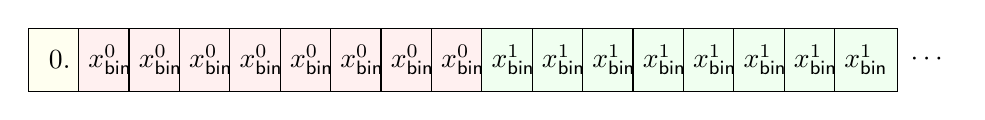
\begin{tikzpicture}[scale=0.8, box/.style={draw,minimum width=0.8cm,minimum height=0.8cm}]
\node[box,fill=lightyellow] at (-0.8,0) {$0.$};
\foreach \x in {0,...,7} {
    \node[box,fill=lightpink] at (\x*0.8,0) {$x^0_{\text{bin}}$};
}
\foreach \x in {8,...,15} {
    \node[box,fill=lightgreen] at (\x*0.8,0) {$x^1_{\text{bin}}$};
}
\node at (13,0) {$\cdots$};
\end{tikzpicture}
\end{center}

First $\tau$ bits encode $x_0$, next $\tau$ bits encode $x_1$, etc.
\end{frame}

\begin{frame}{Historical Background}
Origins:
\begin{itemize}
\item Population demographics model
\item Studied by Robert May (1976)
\item Canonical example of chaos
\end{itemize}

Definition:
\[ z_{k+1} = \mathcal{L}(z_k) = rz_k(1-z_k) \]

We focus on $r=4$ case where:
\begin{itemize}
\item System is fully chaotic
\item Maps [0,1] to itself
\item No stable fixed points
\end{itemize}
\end{frame}

\begin{frame}{Properties of the Logistic Map}
Mathematical structure:
\[ \mathcal{L}(z_k) = 4z_k(1-z_k) \]

Key features:
\begin{itemize}
\item Continuous and differentiable
\item Maximum at $z=1/2$
\item Quadratic nonlinearity
\end{itemize}

\begin{figure}
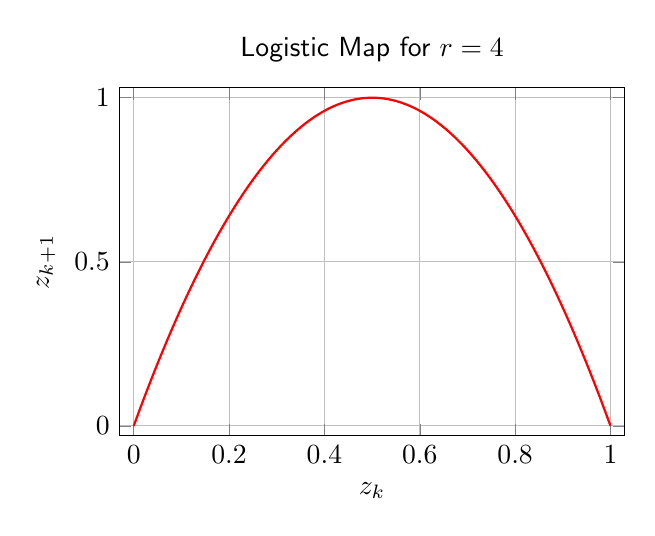
\begin{tikzpicture}
\begin{axis}[
    width=8cm, height=6cm,
    xmin=-0.03, xmax=1.03,
    ymin=-0.03, ymax=1.03,
    xlabel=$z_k$,
    ylabel=$z_{k+1}$,
    grid=both,
    title={Logistic Map for $r=4$}
]
\addplot[domain=0:1,samples=200,thick,red]{4*x*(1-x)};
\end{axis}
\end{tikzpicture}
\end{figure}
\end{frame}

\begin{frame}{Contrast with Dyadic Map}
Comparison:
\begin{columns}
\begin{column}{0.5\textwidth}
Logistic Map $\mathcal{L}$:
\begin{itemize}
\item Smooth
\item Quadratic
\item Continuous
\end{itemize}
\end{column}
\begin{column}{0.5\textwidth}
Dyadic Map $\mathcal{D}$:
\begin{itemize}
\item Piecewise linear
\item Uses modulo
\item Discontinuous
\end{itemize}
\end{column}
\end{columns}

\vspace{0.5cm}
\begin{center}
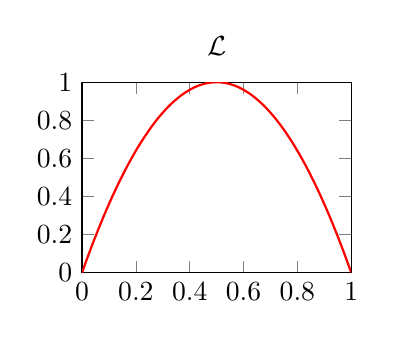
\begin{tikzpicture}
\begin{axis}[
    width=5cm, height=4cm,
    title={$\mathcal{L}$},
    xmin=0, xmax=1,
    ymin=0, ymax=1
]
\addplot[domain=0:1,samples=200,thick,red]{4*x*(1-x)};
\end{axis}
\end{tikzpicture}
\quad
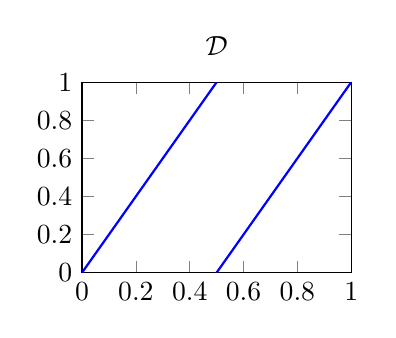
\begin{tikzpicture}
\begin{axis}[
    width=5cm, height=4cm,
    title={$\mathcal{D}$},
    xmin=0, xmax=1,
    ymin=0, ymax=1
]
\addplot[domain=0:0.5,samples=100,thick,blue]{2*x};
\addplot[domain=0.5:1,samples=100,thick,blue]{2*x-1};
\end{axis}
\end{tikzpicture}
\end{center}
\end{frame}

\begin{frame}{The Bridge Function $\phi$}
Definition:
\[ \phi(\alpha) = \sin^2(2\pi\alpha) \]

Properties:
\begin{itemize}
\item Continuous and differentiable
\item Maps [0,1] to [0,1]
\item Periodic with period 1
\item Has continuous inverse
\end{itemize}

\begin{center}
  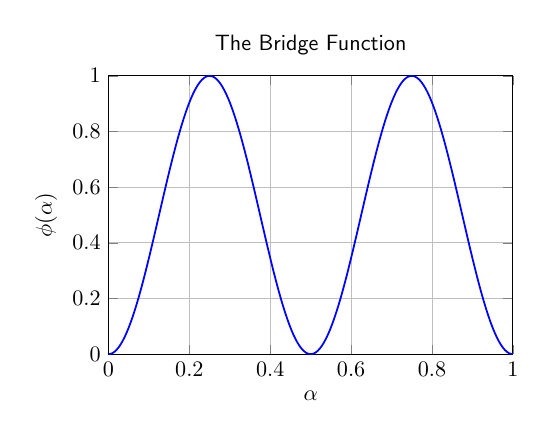
\begin{tikzpicture}[scale=0.8]
\begin{axis}[
    width=8cm, height=6cm,
    xmin=0, xmax=1,
    ymin=0, ymax=1,
    xlabel=$\alpha$,
    ylabel=$\phi(\alpha)$,
    grid=both,
    title={The Bridge Function}
]
\addplot[domain=0:1,samples=200,thick,blue]
    {sin(deg(2*pi*x))^2};
\end{axis}
\end{tikzpicture}
\end{center}
\end{frame}

\begin{frame}{The Inverse Bridge}
Definition:
\[ \phi^{-1}(z) = \frac{\arcsin\sqrt{z}}{2\pi} \]

Properties:
\begin{itemize}
\item Also continuous
\item Maps [0,1] to [0,1/4]
\item Composition yields identity
\end{itemize}

\begin{center}
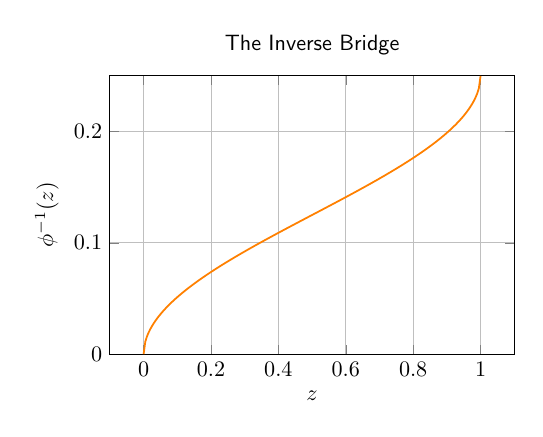
\begin{tikzpicture}[scale=0.8]
\begin{axis}[
    width=8cm, height=6cm,
    xmin=-0.1, xmax=1.1,
    ymin=0, ymax=0.25,   % Adjusted for division by 2π
    xlabel=$z$,
    ylabel=$\phi^{-1}(z)$,
    grid=both,
    title={The Inverse Bridge}
]
\addplot[domain=0:1,samples=200,thick,orange]
    {rad(asin(sqrt(x)))/(2*pi)};  % Division by 2π
\end{axis}
\end{tikzpicture}
\end{center}
\end{frame}

\begin{frame}{The Conjugacy Relation}
Note that 
\[ z_{k+1} = \mathcal{L}(z_k) = 4\phi(\alpha_k)(1 - \phi(\alpha_k)) = 4\sin^2(2\pi\alpha_k)\cos^2(2\pi\alpha_k) = \sin^2(2\pi\cdot 2\alpha_k)\]

Key equation:
\[ \mathcal{L} \circ \phi = \phi \circ \mathcal{D} \]

\begin{center}
\begin{tikzpicture}[node distance=4cm]
\node (a1) {$\alpha_k$};
\node (a2) [right of=a1] {$\alpha_{k+1}$};
\node (z1) [below of=a1,yshift=2cm] {$z_k$};
\node (z2) [below of=a2,yshift=2cm] {$z_{k+1}$};

\draw[->] (a1) -- (a2) node[midway,above] {$\mathcal{D}$};
\draw[->] (z1) -- (z2) node[midway,below] {$\mathcal{L}$};
\draw[->] (a1) -- (z1) node[midway,left] {$\phi$};
\draw[->] (a2) -- (z2) node[midway,right] {$\phi$};
\end{tikzpicture}
\end{center}

Implications:
\begin{itemize}
\item Same dynamics in both spaces
\item Can work in either representation
\item Smooth version available
\end{itemize}
\end{frame}

\begin{frame}{Deriving the Final Formula}

Starting with:
\[ z_k = \phi(\alpha_k) = \sin^2(2\pi\alpha_k) \]

From dyadic map:
\[ \alpha_k = 2^{k\tau}\alpha_0 \bmod 1 \]

Combining gives:
\[ f_\alpha(x) = \sin^2(2^{x\tau}\arcsin\sqrt{\alpha}) \]

This is our elegant final result!
\end{frame}

\begin{frame}[fragile]{Setting Up}
Required imports and precision:
\begin{lstlisting}
from mpmath import mp, pi, sin, asin, sqrt
import numpy as np
from functools import reduce

# Set precision
mp.dps = 1000  # decimal digits
tau = 8        # bits per sample
\end{lstlisting}

Basic helper functions:
\begin{lstlisting}
# Dyadic map
dyadicMap = lambda x: (2 * x) % 1

# Bridge function
phi = lambda alpha: sin(2 * pi * alpha)**2
phiInv = lambda z: asin(sqrt(z)) / (2 * pi)
\end{lstlisting}
\end{frame}

\begin{frame}[fragile]{Binary Conversion}
Converting between representations:
\begin{lstlisting}
def decimalToBinary(decimalInitial):
    return reduce(lambda acc, _: 
        [dyadicMap(acc[0]), acc[1] + ('0' if acc[0] < 0.5 else '1')],
        range(tau), [decimalInitial, ''])[1]

def binaryToDecimal(binaryInitial):
    return reduce(lambda acc, val: 
        acc + int(val[1]) / 2**(val[0] + 1), enumerate(binaryInitial),
        mp.mpf(0.0))
\end{lstlisting}
\end{frame}

\begin{frame}[fragile]{Dataset Processing}
Encoding the dataset:
\begin{lstlisting}
# Convert dataset to binary
binaryInitial = ''.join(map(decimalToBinary, xs))
decimalInitial = binaryToDecimal(binaryInitial)

print('Binary initial:', binaryInitial[:50], '...')
print('Decimal initial:', float(decimalInitial))
\end{lstlisting}

The decoder function:
\begin{lstlisting}
def logisticDecoder(k):
    return sin(2**(k*tau) * asin(sqrt(decimalInitial)))**2

# Recover all samples
decodedValues = [float(logisticDecoder(_)) for _ in range(len(xs))]
\end{lstlisting}
\end{frame}

\begin{frame}[fragile]{Error Checking}
Verify theoretical bounds:
\begin{lstlisting}
# Maximum allowed error
maxError = pi / 2**(tau - 1)

# Check all errors
normalizedErrors = [abs(decoded - true) / maxError 
    for decoded, true in zip(decodedValues, xs)
]

# Verify bounds
assert all(e <= 1.0 for e in normalizedErrors)
print('Maximum normalized error:', max(normalizedErrors))
\end{lstlisting}

Example output:
\begin{lstlisting}[language={}]
Maximum normalized error: 0.8732
All errors within theoretical bound
\end{lstlisting}
\end{frame}

\begin{frame}{Animal Shape Example}
Complete process:
\begin{enumerate}
\item Generate x-coordinates: $x \in [0,\ldots,n]$
\item Choose appropriate $\alpha$ value
\item Compute $y = f_\alpha(x)$ for each x
\item Plot resulting $(x,y)$ pairs
\end{enumerate}

\begin{figure}
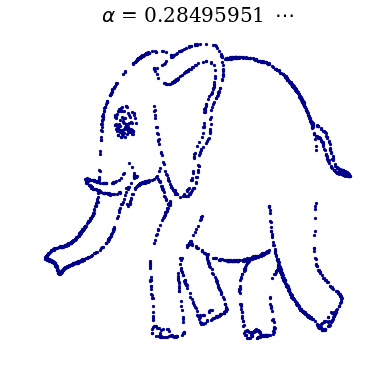
\includegraphics[width=0.24\textwidth]{fig/note01/elephant.png}
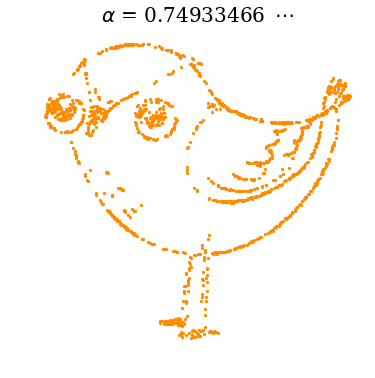
\includegraphics[width=0.24\textwidth]{fig/note01/bird.png}
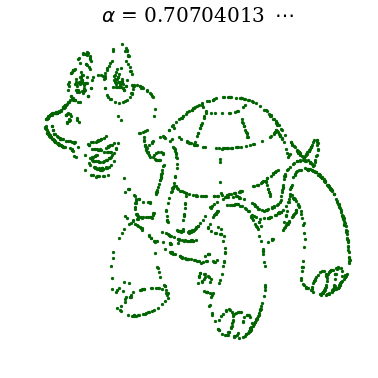
\includegraphics[width=0.24\textwidth]{fig/note01/turtle.png}
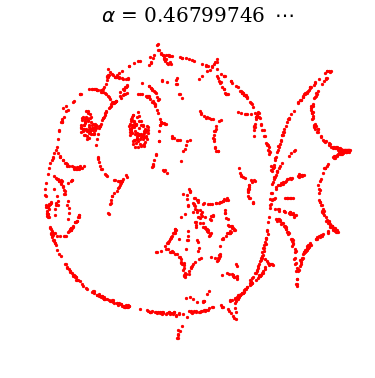
\includegraphics[width=0.24\textwidth]{fig/note01/fish.png}
\caption{Different $\alpha$ values generate different shapes}
\end{figure}
\end{frame}

\begin{frame}{Audio Signal Generation}
Process:
\begin{enumerate}
\item Choose sampling rate (11kHz)
\item Generate time points $t_i$
\item Compute $f_\alpha(i)$ for each $t_i$
\item Scale to audio range [-1,1]
\end{enumerate}

\begin{figure}
\begin{subfigure}{0.48\textwidth}
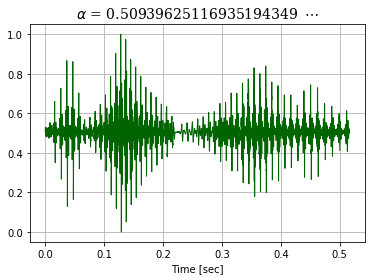
\includegraphics[width=\textwidth]{fig/note01/generated_waveform.png}
\caption{Time domain}
\end{subfigure}
\begin{subfigure}{0.48\textwidth}
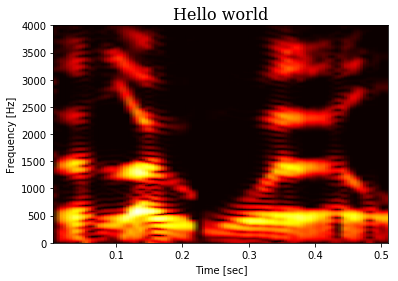
\includegraphics[width=\textwidth]{fig/note01/generated_spectrogram.png}
\caption{Frequency domain}
\end{subfigure}
\caption{"Hello world" audio encoding}
\end{figure}
\end{frame}

\begin{frame}{Image Generation}
CIFAR-10 process:
\begin{enumerate}
\item Generate 3072 values (32×32×3)
\item Reshape into RGB channels
\item Scale to [0,255] range
\item Stack into final image
\end{enumerate}

\begin{figure}
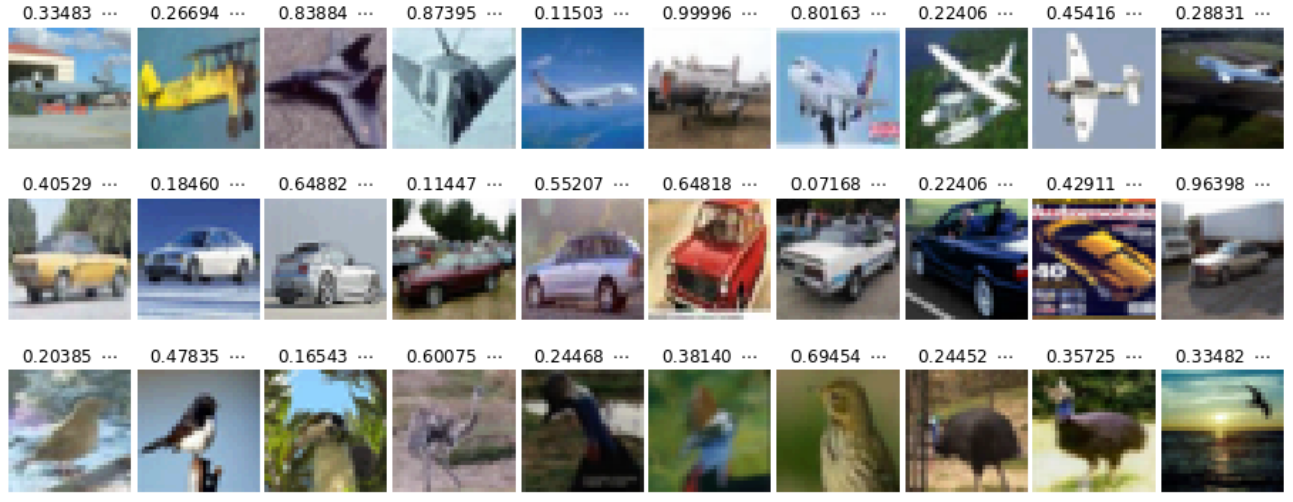
\includegraphics[width=\textwidth]{fig/note01/cifar.png}
\caption{Generated CIFAR-10 style images}
\end{figure}
\end{frame}

\begin{frame}{Generalization Analysis}
Time series example:
\begin{figure}
  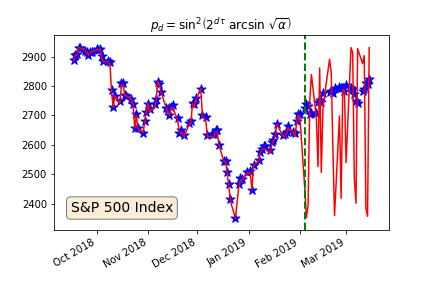
\includegraphics[width=0.9\textwidth]{fig/note01/timeseries.png}
\caption{S\&P 500 predictions showing no generalization}
\end{figure}

Analysis:
\begin{itemize}
\item Perfect fit in training region
\item Random values beyond
\item No true learning occurs
\end{itemize}
\end{frame}

\begin{frame}{Theoretical Implications}
For machine learning:
\begin{itemize}
\item Parameter counting insufficient
\item Need better complexity measures:
    \begin{itemize}
    \item VC dimension
    \item Rademacher complexity
    \item Minimum description length
    \end{itemize}
\item Questions about neural network capacity
\end{itemize}

Mathematical insights:
\begin{itemize}
\item Real numbers contain infinite information
\item Chaos theory in data science
\item Importance of representation
\end{itemize}
\end{frame}

\begin{frame}{Open Questions}
Current questions:
\begin{itemize}
\item Neural network memorization extent
\item Why neural networks generalize
\item Role of optimization algorithms
\end{itemize}

Future directions:
\begin{itemize}
\item New complexity measures
\item Theoretical foundations
\item Practical applications
\end{itemize}
\end{frame}

\begin{frame}{Final Thoughts}
Key takeaways:
\begin{itemize}
\item Single parameter can fit any dataset
\item Connection between chaos and data
\item Questions traditional measures
\item Implications for deep learning
\end{itemize}

Next steps:
\begin{itemize}
\item Develop new theory
\item Better complexity measures
\item Understanding generalization
\end{itemize}

\end{frame}

\end{document}
